\documentclass[../Cours.tex]{subfiles}

\begin{document}

\chapitre{Triangles}

\partie{Constructions}

\definition{Un triangle est une figure plane formée par 3 points et les segments qui les relient.}

\propriete{\centerline{\fbox{Inégalité triangulaire} \vspace{2ex}} Dans un triangle, la longueur d'un côté est toujours inférieure à la somme des longueurs des deux autres côtés.}

\exemple{
    \begin{figure}[!h]
        \centering
        \begin{tikzpicture}
            \coordinate (A) at (0,0);
            \coordinate (B) at (3,1);
            \coordinate (C) at (2,3);
            \draw (A) -- (B) -- (C) -- cycle;
            \node[below] at (A) {$A$};
            \node[below] at (B) {$B$};
            \node[above] at (C) {$C$};
            \node at (7,1+1) {$AB \leq AC + BC$};
            \node at (7,1.5) {$AC \leq AB + BC$};
            \node at (7,1) {$BC \leq AB + AC$};
        \end{tikzpicture}
        \caption{Exemple de triangle $ABC$}
    \end{figure}
}

\consequence{Si au moins une des inégalités n'est pas vraie, alors le triangle ne peut pas être construit.}

\propriete{Il suffit de vérifier l'inégalité correspondant au plus grand côté.}

\propriete{La somme des angles internes d'un triangle vaut \ang{180}.}

\clearpage
\partie{Les différents types de types de triangles et leurs propriétés}
\souspartie{Triangle rectangle}

\definition{Un triangle rectangle possède un angle droit (=\ang{90}).}

\begin{figure}[!h]
    \centering
    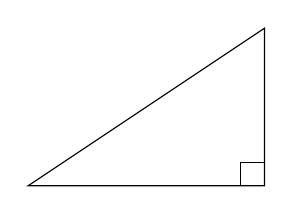
\begin{tikzpicture}
        \draw (0,0) -- (3,0) -- (3,2) -- cycle;
        \draw (3,0) rectangle (2.7,0.3);
    \end{tikzpicture}
\end{figure}


\souspartie{Triangle isocèle}

\definition{Un triangle isocèle possède deux côtés de même longueur.}
\vocabulaire{Le troisième côté est appelé la base du triangle.}
\propriete{Les angles à la base d'un triangle isocèle sont égaux.}

\begin{figure}[h!]
    \centering
    \begin{tikzpicture}
        \draw (0,0) -- (-2,-1) -- (2,-1) -- cycle;
        \node at (-1,-0.5) {||};
        \node at (1,-0.5) {||};
        \draw[fill=rouge,rouge] ($(-2,-1)+(0.5,0)$) arc (0:28:0.5) -- (-2,-1) -- cycle;
        \draw[fill=rouge,rouge] ($(2,-1)+(-0.5,0)$) arc (180:152:0.5) -- (2,-1) -- cycle;
    \end{tikzpicture} 
\end{figure}

\souspartie{Triangle équilatéral}

\definition{Un triangle équilatéral a ses trois côtés de même longueur.}
\propriete{Les trois angles intérieurs sont chacun égaux à \ang{60}.}

\begin{figure}[h!]
    \centering
    \begin{tikzpicture}
        \draw (0,0) -- ($({3*cos(60)},{3*sin(60)})$) -- (3,0) -- cycle;
        \draw[rouge,fill=rouge] (0.3,0) arc (0:60:0.3) -- (0,0) -- cycle;
        \draw[rouge,fill=rouge] (2.7,0) arc (180:120:0.3) -- (3,0) -- cycle;
        \draw[rouge,fill=rouge] ($({2.7*cos(60)},{2.7*sin(60)})$) arc (-120:-60:0.3) -- ($({3*cos(60)},{3*sin(60)})$) -- cycle;
    \end{tikzpicture}
\end{figure}

\partie{Droites remarquables dans un triangle}

\souspartie{Médiatrices}

\definition{La médiatrice d'un segment est la droite qui coupe le segment en son milieu perpendiculairement.}

\illustration{\vspace{-1cm}
\begin{center}
\begin{tikzpicture}
    \draw (0,0) -- (4,0);
    \draw[fill=noir] (0,0) node[below] {$A$} circle (0.05);
    \draw[fill=noir] (4,0) node[below] {$B$} circle (0.05);
    \draw[red] (2,-1.5) -- (2,2);
    \draw[fill=noir] (2,0) rectangle (2.15,0.15);
    \node[rouge] at (1,0) {||};
    \node[rouge] at (3,0) {||};
\end{tikzpicture}
\end{center}
}

\remarque{Dans un triangle, il y a 3 médiatrices.}

\illustration{\vspace{-1cm}
\begin{center}
\begin{tikzpicture}
    \draw[red] (0,0) -- (4,0);
    \draw[dashed,red] (2,-1) -- (2,2);
    \draw[blue] (4,0) -- (3,2);
    \draw[dashed,blue] (3.5,1) -- ++(27:1);
    \draw[dashed,blue] (3.5,1) -- ++(-153:2.5);
    \draw[vert] (3,2) -- (0,0);
    \draw[dashed,vert] (1.5,1) -- ++(123:1);
    \draw[dashed,vert] (1.5,1) -- ++(-57:1.5);
\end{tikzpicture}
\end{center}
}

\propriete{Les trois médiatrices d'un triangle concourent en un point appelé le centre du cercle circonscrit.}

\consequence{Dans un triangle $ABC$, si $M$ est le centre du cercle circonscrit : $$MA = MB = MC$$}

\vspace{-1cm}
\illustration{\vspace{-1cm}
\begin{center}
\begin{tikzpicture}
    \draw[red] (0,0) node[left]{\textcolor{noir}{$A$}} -- (4,0);
    \draw[dashed,red] (2,-1) -- (2,2);
    \draw[blue] (4,0) node[right]{\textcolor{noir}{$B$}} -- (3,2);
    \draw[dashed,blue] (3.5,1) -- ++(27:1);
    \draw[dashed,blue] (3.5,1) -- ++(-153:2.5);
    \draw[vert] (3,2) node[above]{\textcolor{noir}{$C$}} -- (0,0);
    \draw[dashed,vert] (1.5,1) -- ++(123:1);
    \draw[dashed,vert] (1.5,1) -- ++(-57:1.5);
    \draw[fill=black] (2,0.25) circle (0.05);
    \draw (2,0.25) circle (2);
    \node[above right] at (2,0.25) {$M$};
\end{tikzpicture}
\end{center}
}

\souspartie{Hauteurs}

\definition{Dans un triangle, la hauteur d'un côté est la droite perpendiculaire à ce côté et qui passe par le sommet opposé.}

\illustration{\vspace{-1cm}
\begin{center}
\begin{tikzpicture}
    \draw (0,0) node[left]{$A$} -- (4,0) node[right]{$B$} -- (3,2) node[above right]{$C$} -- cycle;
    \draw[red,dashed] (3,-0.5) -- (3,2.5);
    \node[left,red] at (3,1) {$(d)$};
    \node[anchor=west] at (6,1.2) {$(d)$ est la hauteur issue de C.};
    \node[anchor=west] at (6,0.5) {$(d)$ est aussi la hauteur de $[AB]$.};
    \draw[fill=noir] (3,0) rectangle (3.2,0.2);
\end{tikzpicture}
\end{center}
\begin{center}
\begin{tikzpicture}
    \draw (0,0) node[left]{$M$} -- (4,0) node[right]{$N$} -- (1,3) node[above right]{$P$} -- cycle;
    \coordinate (A) at (0,0);
    \coordinate (H) at ($(4,0)!(0,0)!(1,3)$);
    \draw[red,dashed] ($(A)!-0.2!(H)$) -- ($(A)!1.2!(H)$);
    \node[below right,red] at (1,1) {$(d)$};
    \node[anchor=west] at (6,1.2) {$(d)$ est la hauteur issue de $M$.};
    \node[anchor=west] at (6,0.5) {$(d)$ est aussi la hauteur de $[NP]$.};
    \draw[rotate=135,fill=noir] (H) rectangle ($(H)+(0.2,0.2)$);
\end{tikzpicture}
\end{center}
}

\notation{Dans un triangle $ABC$, la hauteur du côté $[AB]$ se nomme aussi la hauteur issue de $C$.}

\propriete{Les trois hauteurs d'un triangle concourent en un point : l'orthocentre.}

\illustration{
\begin{center}
\begin{tikzpicture}[scale=1.5]
    \draw (0,0) node[left]{$A$} coordinate (A) -- (5,0) node[right]{$B$} coordinate (B) -- (1.5,3) node[above left]{$C$} coordinate (C) -- cycle;
    \coordinate (H) at ($(A)!(C)!(B)$);
    \coordinate (I) at ($(A)!(B)!(C)$);
    \coordinate (J) at ($(C)!(A)!(B)$);
    \draw[red, dashed] ($(C)!-0.2!(H)$) -- ($(C)!1.2!(H)$); 
    \draw[red, dashed] ($(B)!-0.2!(I)$) -- ($(B)!1.2!(I)$); 
    \draw[red, dashed] ($(A)!-0.2!(J)$) -- ($(A)!1.2!(J)$);
    \draw[fill=noir] (H) rectangle ($(H)+(0.15,0.15)$);
    \draw[fill=noir,rotate=-25] (I) rectangle ($(I)+(0.15,0.15)$);
    \draw[fill=noir,rotate=-132] (J) rectangle ($(J)+(0.15,0.15)$);
\end{tikzpicture}
\end{center}
}

\clearpage
\EXERCICES 
\begin{questions}
    \exercice Dans chaque cas, dire si le triangle peut être construit ou non.
    \question 
    \begin{center}\vspace{-1ex}
        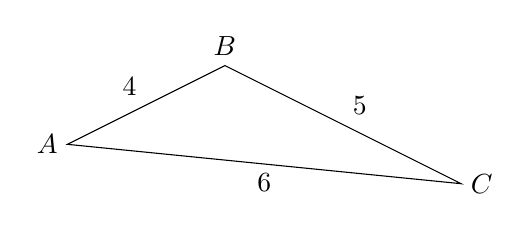
\begin{tikzpicture}
            \draw (0,0) node[left]{$A$} -- ++(2,1) node[above]{$B$} node[midway,anchor=south east]{\qty{4}{\centi\metre}} -- ++(3,-1.5) node[right]{$C$} node[midway,anchor=south west]{\qty{5}{\centi\metre}} -- cycle node[midway,below,anchor=north]{\qty{6}{\centi\metre}};
        \end{tikzpicture}
        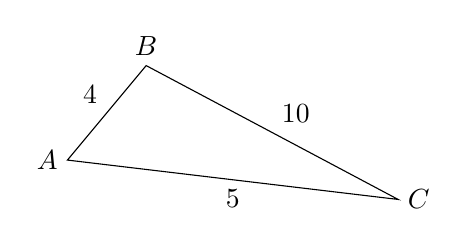
\begin{tikzpicture}
            \draw (0,0) node[left]{$A$} -- ++(1,1.2) node[above]{$B$} node[midway,anchor=south east]{\qty{4}{\centi\metre}} -- ++(3.2,-1.7) node[right]{$C$} node[midway,anchor=south west]{\qty{10}{\centi\metre}} -- cycle node[midway,below,anchor=north]{\qty{5}{\centi\metre}};
        \end{tikzpicture}
        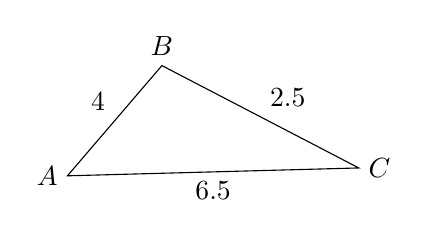
\begin{tikzpicture}
            \draw (0,0) node[left]{$A$} -- ++(1.2,1.4) node[above]{$B$} node[midway,anchor=south east]{\qty{4}{\centi\metre}} -- ++(2.5,-1.3) node[right]{$C$} node[midway,anchor=south west]{\qty{2.5}{\centi\metre}} -- cycle node[midway,below,anchor=north]{\qty{6.5}{\centi\metre}};
        \end{tikzpicture}
    \end{center}
    \question $AB=11$, $AC=14$ et $BC=8$
    \question $AB=\qty{3.2}{\metre}$, $BC=\qty{9.8}{\metre}$, $AC=\qty{6.4}{\metre}$
    \question $ABC$ est un triangle équilatéral avec $AB=4$
    \question $ABC$ est un triangle isocèle en B avec $AB=\qty{3}{\centi\metre}$ et $AC=\qty{5}{\centi\metre}$
    \question $ABC$ est un triangle isocèle en C avec $AB=\qty{12}{\milli\metre}$ et $AC=\qty{4}{\milli\metre}$

    \exercice 
\end{questions}

\renewcommand\tabularxcolumn[1]{m{#1}}
\begin{tabularx}{\textwidth}{C|C}\hline
    \makecell{La hauteur du côté $[AB]$ \\ la hauteur issue de $C$} & 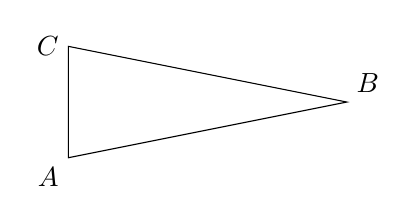
\begin{tikzpicture}[rotate=-45]
        \coordinate (A) at (0,0);
        \coordinate (B) at (2,3);
        \coordinate (C) at (-1,1);
        \draw (A) node[below left]{$A$} -- (B) node[above right]{$B$} -- (C) node[left]{$C$} -- cycle;
    \end{tikzpicture} \\\hline
    .... & \begin{tikzpicture}[rotate=-35]
        \coordinate (A) at (0,0);
        \coordinate (B) at (2,3);
        \coordinate (C) at (-1,1);
        \draw (A) node[below left]{$A$} -- (B) node[above right]{$B$} -- (C) node[left]{$C$} -- cycle;
        \coordinate (H) at ($(B)!(A)!(C)$);
        \draw[dashed] ($(A)!-0.2!(H)$) -- ($(A)!1.5!(H)$);
    \end{tikzpicture} \\\hline
    .... & \begin{tikzpicture}[rotate=-35]
        \coordinate (A) at (0,0);
        \coordinate (B) at (3,2);
        \coordinate (C) at (-1,1);
        \draw (A) node[below left]{$A$} -- (B) node[above right]{$B$} -- (C) node[left]{$C$} -- cycle;
        \coordinate (I) at ($(B)!0.5!(C)$);
        \coordinate (v) at (1,-4);
        \draw[dashed] ($(I)-0.5*(v)$) -- ($(I)+0.5*(v)$);
    \end{tikzpicture} \\\hline
    La médiatrice de $[AC]$ & 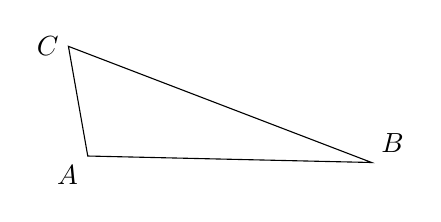
\begin{tikzpicture}[rotate=-35]
        \coordinate (A) at (0,0);
        \coordinate (B) at (3,2);
        \coordinate (C) at (-1,1);
        \draw (A) node[below left]{$A$} -- (B) node[above right]{$B$} -- (C) node[left]{$C$} -- cycle;
    \end{tikzpicture} \\\hline
    Les trois médiatrices de $ABC$ & \begin{tikzpicture}[rotate=-25]
        \coordinate (A) at (0,-1);
        \coordinate (B) at (3,1.5);
        \coordinate (C) at (-1,0);
        \draw (A) node[below left]{$A$} -- (B) node[above right]{$B$} -- (C) node[left]{$C$} -- cycle;
        \coordinate (I) at ($(B)!0.5!(C)$);
        \coordinate (v) at (1.5,-4);
        \draw[dashed] ($(I)-0.5*(v)$) -- ($(I)+0.5*(v)$);
    \end{tikzpicture} \\\hline
    Les trois hauteurs de $ABC$ & \begin{tikzpicture}[rotate=-25]
        \coordinate (A) at (-0.6,-1.8);
        \coordinate (B) at (3,1.5);
        \coordinate (C) at (-2,0);
        \draw (A) node[below left]{$A$} -- (B) node[above right]{$B$} -- (C) node[left]{$C$} -- cycle;
        \coordinate (H) at ($(B)!(A)!(C)$);
        \draw[dashed] ($(A)!-0.2!(H)$) -- ($(A)!1.5!(H)$);
    \end{tikzpicture} \\\hline
\end{tabularx}

\end{document}